\documentclass[12pt]{report}

% Packages
\usepackage{acronym}
\usepackage{amsmath}
\usepackage{amsthm}
\usepackage{amsfonts}
\usepackage{epigraph}
\usepackage{geometry}
\usepackage{graphicx}
%\usepackage{mdframed}
\usepackage{titlesec}
\usepackage{caption}
\usepackage{listings}
\usepackage{xcolor}
\usepackage{siunitx}
\usepackage{enumitem}
\usepackage{pdfpages}
\usepackage[utf8]{inputenc}
\usepackage{fancyhdr}
\usepackage{transparent}
\usepackage[hidelinks, colorlinks=true, linkcolor=blue, urlcolor=blue, citecolor=blue]{hyperref}
\usepackage[backend=biber, style=ieee]{biblatex}
%\addbibresource{cdt_app.bib}

% Acronym set-up
% Command to insert acronyms with a temporary color change
\newcommand{\myAcro}[1]{{\hypersetup{linkcolor=black}\acl{#1}}} % For acronym list (full form)
\newcommand{\myAcroLink}[1]{{\hypersetup{linkcolor=black}\acs{#1}}}

% Document geometry setup
\geometry{
    a4paper,
    margin=2cm,
    top=1cm,    % Adjust top margin
    bottom=1cm,  % Adjust bottom margin
    headheight=14.5pt,
    includeheadfoot
}

\pagestyle{fancy} % Use fancy style for all pages
\fancyhf{} % Clear all header and footer fields

% Header
\fancyhead[L]{{\transparent{0.5}Chapter \udlchap{} Questions}} % Left header
\fancyhead[R]{{\transparent{0.5}wp289}} % Right header

% Footer
\fancyfoot[L]{\transparent{0.5}Understanding Deep Learning} % Left footer
\fancyfoot[R]{\transparent{0.5}\thepage} % Right footer

% Define line thickness
\renewcommand{\headrulewidth}{0.4pt}
\renewcommand{\footrulewidth}{0.4pt}

% Redefining plain page style if needed
\fancypagestyle{plain}{ % Applies to chapter beginnings and similar
  \fancyhf{} % clear all header and footer fields for plain style
  \renewcommand{\headrulewidth}{0.4pt}
  \renewcommand{\footrulewidth}{0.4pt}
  \fancyhead[L]{{\transparent{0.5}Chapter \udlchap{}Questions}}
  \fancyhead[R]{{\transparent{0.5}wp289}}
  \fancyfoot[L]{\transparent{0.5}Understanding Deep Learning}
  \fancyfoot[R]{\transparent{0.5}\thepage}
}

% Customise Chapter Headings
\titleformat{\chapter}
    {\normalfont\LARGE\bfseries}
    {\thechapter.}
    {1em}
    {}
\titlespacing*{\chapter}{0pt}{-20pt}{\baselineskip}

% Customise section spacing
\titlespacing*{\section}{0pt}{\baselineskip}{0.5\baselineskip}

% Adjusting space around figures
\setlength{\floatsep}{5pt}
\setlength{\textfloatsep}{5pt}

% Adjusting caption spacing
\captionsetup{aboveskip=5pt, belowskip=5pt}

% Format paragraphs
\setlength{\parindent}{0pt}
\setlength{\parskip}{1em}  % Adjust the value as needed

% Adjust list spacing
%\setlist[enumerate]{before=\vspace{0.5em}, after=\vspace{0.5em}}
\setlist[enumerate]{before=\vspace{-0.5\baselineskip}, after=\vspace{-0.5\baselineskip}}

% Customise question boxes
\usepackage[framemethod=TikZ]{mdframed}
\mdfsetup{
    backgroundcolor=gray!20,
    innertopmargin=10pt,
    innerbottommargin=10pt,
    skipbelow=0pt 
}

\def\udlchap{5}
\renewcommand{\thesubsection}{Problem \udlchap.\arabic{subsection}}

%%%%%%%%%%%%%%%%%%%%%%%%%%%%%%%%%%%%%%%%%%%%%%%%%%%%%%%%%

\begin{document}

\section*{Chapter 5: Loss functions}

\subsection{}
\begin{mdframed}
    Show that the logistic sigmoid function sig[$z$] maps $z = -\infty$ to 0, $z=0$ to 0.5, and $z = \infty$ to 1, where:
    \begin{equation*}
        \text{sig}[z] = \frac{1}{1+\text{exp}[-z]}
    \end{equation*}
\end{mdframed}

When $z = -\infty$:

\begin{equation*}
    \text{sig}[-\infty] = \frac{1}{1+\text{exp}[\infty]} = \frac{1}{1+\text{exp}[\infty]} = \frac{1}{\infty} = 0
\end{equation*}

When $z=0$:

\begin{equation*}
    \text{sig}[-\infty] = \frac{1}{1+\text{exp}[0]} = \frac{1}{1+\text{exp}[0]} = \frac{1}{1 + 1} = \frac{1}{2}
\end{equation*}

When $z=\infty$:

\begin{equation*}
    \text{sig}[\infty] = \frac{1}{1+\text{exp}[-\infty]} = \frac{1}{1+\text{exp}[-\infty]} = \frac{1}{1+0} = 1
\end{equation*}



\subsection{}
\begin{mdframed}
    The loss $L$ for binary classification for a single training pair $\{\mathbf{x},y\}$ is:
    \begin{equation*}
        L = -1(1-y) \text{log}\left[1- \text{sig}[f[\mathbf{x}, \phi]]\right] -y\text{log}\left[\text{sig}[f[\mathbf{x}, \phi]]\right]
    \end{equation*}
    where sig[$\bullet$] is defined above. Plot this loss as a function of the transformed network output $\text{sig}[f[\mathbf{x},\phi]] \in [0,1]$ when the training label $y=0$ and when $y=1$.
\end{mdframed}

\begin{figure}[h]
    \centering
    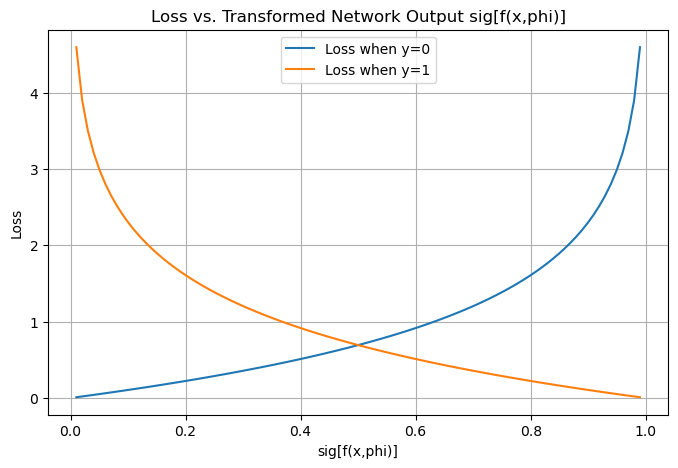
\includegraphics[width=0.6\textwidth]{q5_2.png}
    \label{fig:q5_2}
\end{figure}

\subsection{}
\begin{mdframed}
    Suppose we want to build a network that predicts the direction y in radians of the prevailing wind based on local measurements of barometric pressure $\mathbb{x}$. A suitable distribution over circular domains is the von Mises distribution (figure 5.13 from book)
    \begin{equation*}
        P(y|\mu,\kappa) = \frac{\text{exp}[\kappa\text{cos}(y-\mu)}{2\pi \cdot \text{Bessel}_{0}[\kappa]}
    \end{equation*}
    where $\mu$ is a measure of the mean direction and $\kappa$ is a measure of the concentration (i.e., the inverse of the variance). The term $\text{Bessel}_{0}[\kappa]$ is a modified Bessel function of order 0. Use the recipe from section 5.2 to develop a loss function for learning the parameter $\mu$ of a model $f[\mathbf{x},\phi]$ to predict the most likely wind direction. your solution should treat the concentration $\kappa$ as constant. How would you perform inference?
\end{mdframed}

To train the model, find the network paramaters $\hat{\phi}$ that minimise the negative log-likelihood (NLL) function over the training set. The NLL for the above distribution can be written as:

\begin{align*}
    L & = \sum^{I}_{i=1} - \text{log}\left[\frac{\text{exp}[\kappa\text{cos}(y_{i}-f[\mathbf{x}_{i}, \phi]]}{2\pi \cdot \text{Bessel}_{0}[\kappa]}\right] \\
      & = -\kappa\text{cos}(y_{i}-f[\mathbf{x}_{i}, \phi]) + \text{log}[\text{Bessel}_{0}[\kappa]]
\end{align*}

Since $\kappa$ is constant, the above loss function can be simplified to:

\begin{equation*}
    L = -\text{cos}(y_{i}-f[\mathbf{x}_{i}, \phi])
\end{equation*}

To perform inference you would take the maximum of the distribution which is just the predicted parameter $\mu$. This may be out of the range $[-\pi,\pi]$, in which case we would add/remove multiples of $2\pi$ until it is in the original range.

\subsection{}

\begin{mdframed}
    Sometimes the outputs y for input $\mathbf{x}$ are multimodal; there is more than one valid prediction for a given input. Here, we might use a weighted sum of normal components as the distribution over the output. This is known as a \textit{mixture of Gaussians} model. For example, a mixture of two Gaussians has parameters $\boldsymbol{\theta} = \{\lambda,\mu_{1}, \sigma_{1}^{2},\mu_{2}, \sigma_{2}^{2}$:

    \begin{equation*}
        P(y|\lambda,\mu_{1}, \sigma_{1}^{2},\mu_{2}, \sigma_{2}^{2}) = \frac{\lambda}{\sqrt{2\pi\sigma_{1}^{2}}}\text{exp}\left[\frac{-(y-\mu_{1})^{2}}{2\sigma_{1}^{2}}\right] + \frac{1-\lambda}{\sqrt{2\pi\sigma_{2}^{2}}}\text{exp}\left[\frac{-(y-\mu_{2})^{2}}{2\sigma_{2}^{2}}\right]
    \end{equation*}

    where $\lambda \in [0,1]$ controls the relative weight of the two components, which have means $\mu_{1}, \mu_{2}$ and variances $\sigma_{1}^{2}, \sigma_{2}^{2}$, respectively. This model can represent a distribution with two peaks or a distribution with one peak but a more complex shape.

    Use the recipe from section 5.1 to construct a loss function for training a model $\mathbf{f}[\mathbf{x}, \phi]$ that takes input $x$, has parameter $\phi$, and predicts a mixture of two Gaussians. The loss should be based on $I$ training data pairs $\{x_{i},y_{i}\}$. What problems do you foresee when performing inference?
\end{mdframed}

The NLL for the above distribution can be written as, assuming $\mathbf{f}_{d}[\mathbf{x}_{i}, \phi]$ is the $d^{th}$ set of network outputs:

\begin{equation*}
    L = \sum^{I}_{i=1} - \text{log}\left[\frac{\text{sig}[\mathbf{f}_{1}[\mathbf{x}_{i}, \phi]]}{\sqrt{2\pi\mathbf{f}_{3}[\mathbf{x}_{i}, \phi]^{2}}}\text{exp}\left[\frac{-(y_{i}-\mathbf{f}_{2}[\mathbf{x}_{i}, \phi])^{2}}{2\mathbf{f}_{3}[\mathbf{x}_{i}, \phi]^{2}}\right] + \frac{1-\text{sig}[\mathbf{f}_{1}[\mathbf{x}_{i}, \phi]]}{\sqrt{2\pi\mathbf{f}_{4}[\mathbf{x}_{i}, \phi]^{2}}}\text{exp}\left[\frac{-(y_{i}-\mathbf{f}_{4}[\mathbf{x}_{i}, \phi])^{2}}{2\mathbf{f}_{4}[\mathbf{x}_{i}, \phi]^{2}}\right]\right]
\end{equation*}

Inference is slightly more tricky as there is no simple closed form expression for the mode of this distribution. We might have to find it using optimization

\subsection{}
\begin{mdframed}
    Consider extending the model from problem 5.3 to predict the wind direction using a mixture of two von Mises distributions. Write an expression for the likelihood $P(y|\boldsymbol{\theta})$ for this model. How many outputs will the network need to produce?
\end{mdframed}

A mixture of two von Mises distributions can be written as follows:

\begin{equation*}
    P(y|\mu,\kappa) = \pi \cdot\frac{\text{exp}[\kappa\text{cos}(y-\mu_{1})}{2\pi \cdot \text{Bessel}_{0}[\kappa]} + (1-\pi)\cdot\frac{\text{exp}[\kappa\text{cos}(y-\mu_{2})}{2\pi \cdot \text{Bessel}_{0}[\kappa]}
\end{equation*}

The network would need to produce three outputs: the mean for the first von Mises distribution ($\mu_{1}$), the mean for the second von Mises distribution ($\mu_{2}$), and the mixing coefficient $\pi$.

\subsection{}
\begin{mdframed}
    Consider building a model to predict the number of pedestrians $y \in \{0,1,2,\dots\}$ that will pass a given point in the city in the next minute, based on data $x$ that contains information about the time of day, the longitude and latitude, and the type of neighborhood. A suitable distribution for modeling counts is the Poisson distribution (figure 5.15 from book). This has a single parameter $\lambda > 0$ called the rate that represents the mean of the distribution. The distribution has probability density function:

    \begin{equation*}
        P(y = k) = \frac{\lambda^{k}e^{-\lambda}}{k!}
    \end{equation*}

    Design a loss function for this model assuming we have access to $I$ training pairs $\{\mathbf{x}_{i},y_{i}\}$.
\end{mdframed}

In this context $\lambda$ is not fixed, but a function of the data: $\lambda = f[\mathbf{x}, \phi]$. The NLL function for a single observation $(\mathbf{x}, y)$ is given by:

\begin{equation*}
    -\text{log}\left(\frac{\lambda^{k}e^{-\lambda}}{k!}\right) = -k\text{log}(\lambda) + \lambda + \text{log}(k!)
\end{equation*}

Since $k!$ is a constant for all true counts $k$, it can be ignored. To find the loss over all $I$ training pairs, take the sum of the negative log-likelihoods for all observations:

\begin{equation*}
    L = \sum^{I}_{i=1}[-y_{i}\text{log}(\lambda_{i}) + \lambda_{i}]
\end{equation*}

\subsection{}
\begin{mdframed}
    Consider a multivariate regression problem where we predict 10 outputs so $\mathbf{y} \in \mathbb{R}^{10}$, and model each with an independent normal distribution where the means $\mu_{d}$ are predicted by the network, and variances $\sigma^{2}$ are all the same. Write an expression for the likelihood $P(\mathbf{y}|\mathbf{f}[\mathbf{x},\boldsymbol{\phi}])$ for this model. Show that minimizing the negative log-likelihood of this model is still equivalent to minimizing a sum of squared terms if we don’t estimate the variance $\sigma^{2}$.
\end{mdframed}

Given this setup, the likelihood of observing a particular $\mathbf{y}$ given model predictions $\mathbf{f}[\mathbf{x},\boldsymbol{\phi}]$, where $\phi$ are the parameters of the model, can be expressed as:

\begin{equation*}
    P(\mathbf{y}|\mathbf{f}[\mathbf{x},\boldsymbol{\phi}]) =\prod_{d=1}^{10}\frac{1}{\sqrt{2\pi\sigma^{2}}}\text{exp}\left[\frac{-(y_{d}-\mu_{d})^{2}}{2\sigma^{2}}\right]
\end{equation*}

The NLL is therefore:

\begin{align*}
    -\text{log}P(\mathbf{y}|\mathbf{f}[\mathbf{x},\boldsymbol{\phi}]) & = -\text{log}\left(\prod_{d=1}^{10}\frac{1}{\sqrt{2\pi\sigma^{2}}}\text{exp}\left[\frac{-(y_{d}-\mu_{d})^{2}}{2\sigma^{2}}\right]\right) \\
                                                                      & = -\sum_{d=1}^{10}\text{log}\left(\frac{1}{\sqrt{2\pi\sigma^{2}}}\text{exp}\left[\frac{-(y_{d}-\mu_{d})^{2}}{2\sigma^{2}}\right]\right)  \\
                                                                      & = \sum_{d=1}^{10}\frac{(y_{d}-\mu_{d})^{2}}{2\sigma^{2}}                                                                                 \\
                                                                      & = \sum_{d=1}^{10}(y_{d}-\mu_{d})^{2}
\end{align*}

which is equivalent to minimising the sum of squared term (if we don't estimate the variance $\sigma^{2}$).

\subsection{}
\begin{mdframed}
    Construct a loss function for making multivariate prediction $\mathbf{y}$ based on independent normal distributions with different variances $\sigma^{2}_{d}$ for each dimension. Assume a heteroscedastic model so that both means $\mu_{d}$ and variances $\sigma^{2}_{d}$ vary as a function of the data
\end{mdframed}

\begin{equation*}
    L = -\sum_{i=1}^{I}\text{log}\left(\prod_{d=1}^{D_{i}}\frac{1}{\sqrt{2\pi\mathbf{f}_{2d}[\mathbf{x}_{i},\boldsymbol{\phi}]^{2}}}\text{exp}\left[\frac{-(y_{id}-\mathbf{f}_{1d}[\mathbf{x}_{i},\boldsymbol{\phi}])^{2}}{2\mathbf{f}_{2d}[\mathbf{x}_{i},\boldsymbol{\phi}]^{2}}\right]\right)
\end{equation*}

\subsection{}
\begin{mdframed}
    Consider a multivariate regression problem in which we predict the height of a person in meters and their weight in kilos from data $\mathbf{x}$. Here, the units take quite different ranges. What problems do you see this causing? Propose two solutions to these problems.
\end{mdframed}

The height uses different units than the weight and the numbers will be smaller. Consequently, the least squares loss will focus much more on the weight than the height. Two possible solutions are (i) to rescale the outputs so that they have the same standard deviation, build a model that predicts the rescaled outputs, and scale them back after inference or (ii) learn a separate variance for the two dimensions so that the model can automatically take care of this. The second approach can be done in either a homoscedastic or heteroscedastic context.

\subsection{}
\begin{mdframed}
    Extend the problem from 5.3 to predict both the wind direction and the wind speed and define the associated loss function.
\end{mdframed}

\begin{equation*}
    L = \sum^{I}_{i=1} - \text{log}\left[\frac{\text{exp}[\mathbf{f}_{2}[\mathbf{x}_{i}, \phi]\text{cos}(y_{i}-\mathbf{f}_{1}[\mathbf{x}_{i}, \phi]]}{2\pi \cdot \text{Bessel}_{0}[\mathbf{f}_{2}[\mathbf{x}_{i}, \phi]]}\right]
\end{equation*}

\end{document}
